\documentclass[10pt,twocolumn,letterpaper]{article}

%%%%%%%%% PAPER TYPE  - PLEASE UPDATE FOR FINAL VERSION
% \usepackage{iccv}              % To produce the CAMERA-READY version
\usepackage[review]{iccv}      % To produce the REVIEW version
% \usepackage[pagenumbers]{iccv} % To force page numbers, e.g. for an arXiv version

% --- CORE PACKAGES ---
\usepackage{times}
\usepackage{epsfig}
\usepackage{graphicx}
\usepackage{amsmath}
\usepackage{amssymb}
\usepackage{booktabs}
\usepackage{enumitem}
\usepackage{microtype}

\definecolor{iccvblue}{rgb}{0.21,0.49,0.74}
\usepackage[pagebackref,breaklinks,colorlinks,allcolors=iccvblue]{hyperref}

% --- CUSTOM COMMANDS ---
\newcommand{\deltaMetric}{\Delta}
\newcommand{\textSub}[1]{_{\text{#1}}}

\setlength{\textfloatsep}{6pt plus 1pt minus 1pt}
\setlength{\floatsep}{5pt plus 1pt minus 1pt}
\setlength{\intextsep}{5pt plus 1pt minus 1pt}

% Support for easy cross-referencing
\usepackage[capitalize]{cleveref}
\crefname{section}{Sec.}{Secs.}
\Crefname{section}{Section}{Sections}
\Crefname{table}{Table}{Tables}
\crefname{table}{Tab.}{Tabs.}

%%%%%%%%% PAPER ID  - PLEASE UPDATE
\def\paperID{*****} % *** Enter the Paper ID here
\def\confName{ICCV}
\def\confYear{2025}

\begin{document}

%%%%%%%%% TITLE
\title{Dense Caption Reconstruction: Quantifying Causal Narrative Inference\\and Visual Decoupling in Video Language Models}

\author{Anonymous Authors\\
Paper ID \paperID
}

\maketitle

%%%%%%%%% ABSTRACT
\begin{abstract}
Current Video-Language Models (Video-LLMs) routinely process dense visual frames as an uncompressed, uniform token sequence, incurring severe computational costs regardless of the video's underlying information density. Yet, many real-world physical events follow structured causal scripts that can be inferred without continuous optical observation. In this paper, we establish a diagnostic framework for \textbf{Dense Caption Reconstruction} to measure the boundary between \textbf{symbolic narrative inference} (what causally must occur) and \textbf{visual perception} (what optical details actually occurred). Evaluating on a 100-video benchmark across six diverse domains, we compare whole-window LLM reasoning (Llama-3.1-8B), iterative cloze completion (Phi-3-mini-4k), and non-parametric visual vector interpolation across multi-second masked gaps (\(W=3\)).
Our empirical analysis reveals two fundamental phenomena:
(1) \textbf{The Modality Decoupling Law}: while visual vector continuity collapses catastrophically under optical motion variance (\(r = -0.865, p < 0.0001\)), LLM narrative deduction is statistically invariant to camera and optical dynamics (\(r = -0.001, p = 0.99\)).
(2) \textbf{Scale-Induced Surprisal Immunity}: smaller SLMs (3.8B) suffer steep performance degradation under high a priori caption surprisal (\(r = -0.641, p < 0.0001\)), whereas 8B-scale parametric models exhibit complete statistical immunity (\(r = +0.028, p = 0.79\)), sustaining an overall Mean Reciprocal Rank (MRR) of 0.558 (+26.5\% relative gain over Phi-3).
These findings demonstrate that symbolic narrative logic reliably bridges visual blind spots, offering concrete mathematical criteria for dynamic token pruning and temporal compression in next-generation multimodal architectures.
\end{abstract}

%%%%%%%%% BODY TEXT
\section{Introduction}
\label{sec:intro}

Modern Video-Language Models (Video-LLMs)~\cite{lin2023video,maaz2023video} have achieved impressive capabilities in video question answering and temporal grounding. However, their computational architecture relies almost exclusively on dense, brute-force visual encoding: high-rate video frames are projected into continuous embedding spaces and consumed uniformly by transformer backbones. This design overlooks a fundamental property of human physical reality: \textit{narrative predictability}. 

\begin{figure*}[t]
  \centering
  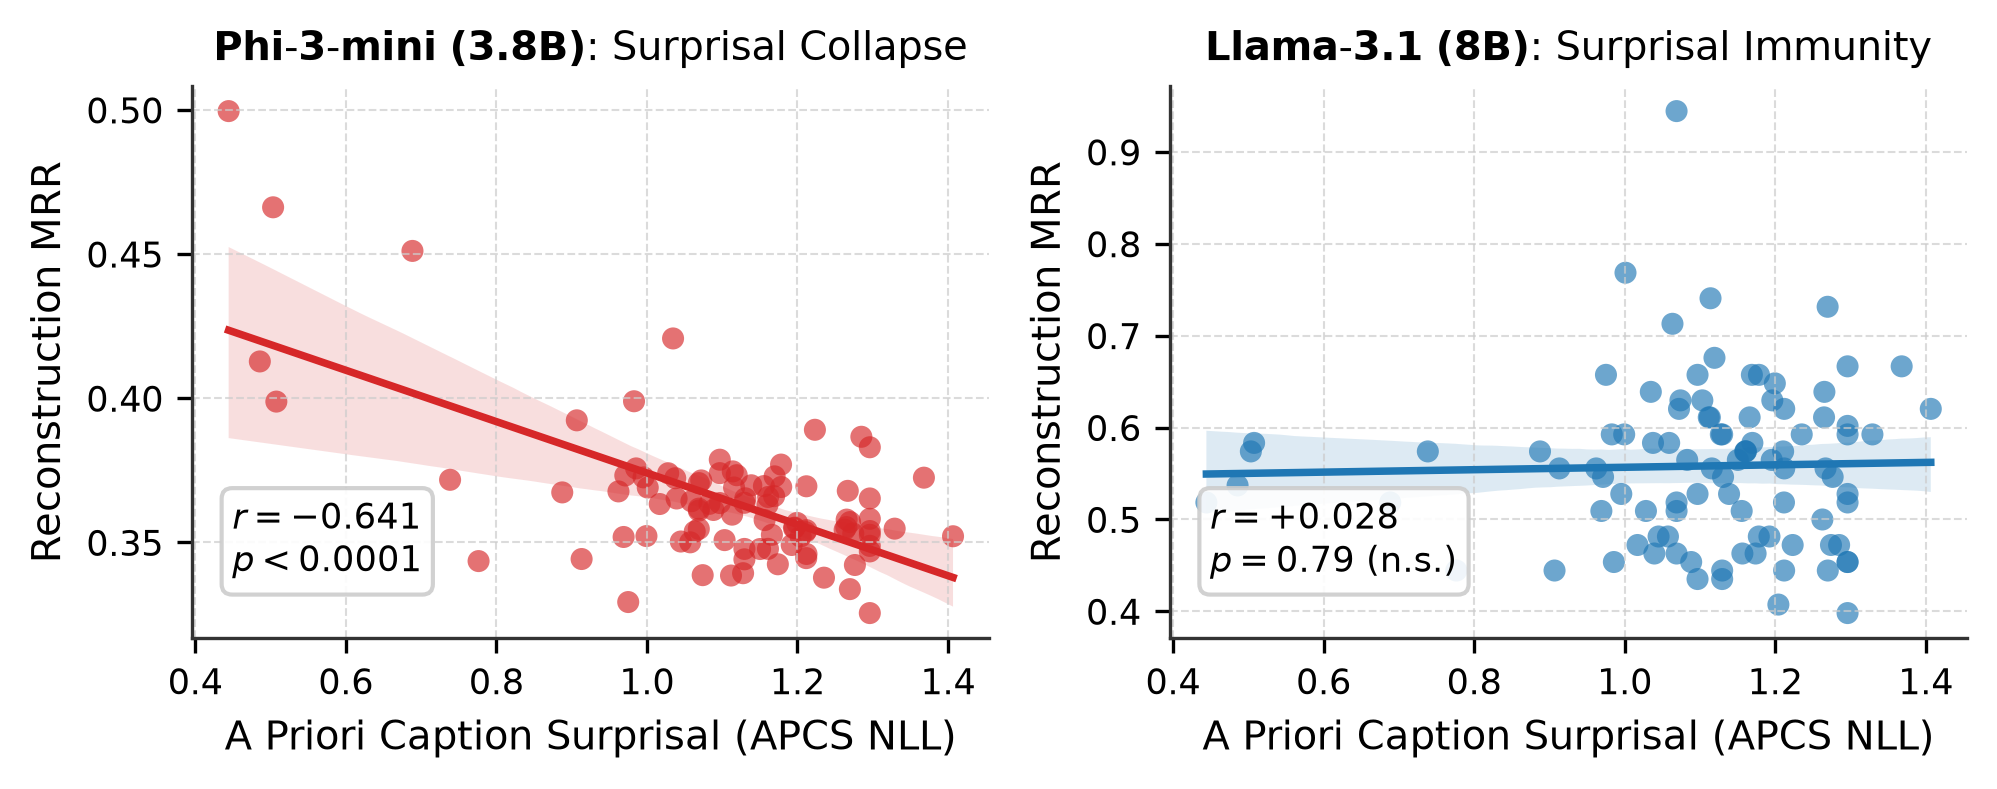
\includegraphics[width=0.98\textwidth]{figures/fig1_surprisal_immunity.png}
  \vspace{-2mm}
  \caption{\textbf{Scale-Induced Surprisal Immunity.} Under increasing a priori caption surprisal (APCS NLL), the smaller 3.8B model (Phi-3-mini) collapses (\(r = -0.641, p < 0.0001\)), whereas the 8B model (Llama-3.1) exhibits complete statistical immunity (\(r = +0.028, p = 0.79\)), proving that larger parametric capacity is essential for out-of-distribution causal reasoning.}
  \label{fig:surprisal_immunity}
  \vspace{-3mm}
\end{figure*}

Consider a cooking sequence where an instructor slices vegetables and later plates a cooked stir-fry. Even if intermediate camera footage is missing or blurred, any competent observer—and indeed, any large language model with sufficient world knowledge—can deduce with high confidence that the chef heated the wok, sauteed the aromatics, and added the vegetables. The precise visual pixels (such as optical flare or hand tremor) are \textit{stochastic residuals}, but the \textit{causal narrative} is procedurally deterministic. Conversely, in unconstrained wildlife footage, a predator's sudden change in direction cannot be deduced from prior trajectory alone and demands continuous optical observation.

To rigorously interrogate this trade-off, we formalize the task of \textbf{Dense Caption Reconstruction}. Given a sequence of dense semantic events where an entire temporal window of consecutive intervals is masked out, we evaluate whether language models can reconstruct the missing narrative sequence purely from temporal context, and compare this against non-parametric visual vector continuity.

Through systematic cross-evaluation of prior informational metrics and post-reconstruction performance across 100 wild videos, this work delivers three primary contributions:
\begin{itemize}[leftmargin=*,noitemsep,topsep=2pt]
    \item \textbf{Modality Decoupling Law}: We prove mathematically and empirically that visual continuity and symbolic language reasoning are completely orthogonal. Visual interpolation collapses under optical motion variance (\(r = -0.865\)), whereas language models reason causally regardless of camera dynamics (\(r = -0.001\)).
    \item \textbf{Surprisal Immunity at Scale}: We demonstrate that while compact 3.8B SLMs collapse when scene descriptions deviate from stereotypical phrases (\(r = -0.641\)), 8B models possess the parametric world knowledge to reconstruct high-entropy events without degradation (\(r = +0.028\)).
    \item \textbf{Diagnostic Bottleneck Metrics}: We show that minimum cosine similarity (\(\cos\text{Sim}_{\min}\)) serves as an acute indicator of localized temporal rupture, and uncover that backward causal deduction makes opening video sequences (\(i=0\)) the most accurately reconstructible positions on the benchmark.
\end{itemize}

%-------------------------------------------------------------------------
\section{Methodology}
\label{sec:method}

\subsection{Problem Formulation}
Let a video \(V\) be represented as an ordered sequence of \(T\) synchronized semantic intervals:
\begin{equation}
    V = \{(v_t, c_t)\}_{t=1}^T
\end{equation}
where \(v_t \in \mathbb{R}^D\) denotes the visual embedding of interval \(t\) (extracted via CLIP-ViT~\cite{radford2021learning}), and \(c_t\) denotes its dense natural language caption. We define a masked temporal window \(M \subset \{1, \dots, T\}\) of width \(W = |M|\). The observed context is \(O = \{t \in \{1, \dots, T\} \mid t \notin M\}\). The objective is to reconstruct the semantic embeddings of the unobserved intervals \(\{\hat{e}_t\}_{t \in M}\).

\subsection{Reconstruction Pathways}

\noindent \textbf{Whole-Window Parametric Reasoning:}
We condition an instruction-tuned LLM (Llama-3.1-8B-Instruct~\cite{dubey2024llama3}) on the complete observed caption history \(\{c_t\}_{t \in O}\) with explicit temporal gap markers indicating the timestamp span. The model generates the entire sequence of missing captions \(\{\hat{c}_t\}_{t \in M}\) simultaneously. Reconstructed captions are then mapped to semantic embeddings via a frozen text encoder: \(\hat{e}\textSub{text}(t) = \mathcal{E}\textSub{text}(\hat{c}_t)\).

\noindent \textbf{Iterative Cloze Baseline:}
As an SLM baseline, we evaluate Phi-3-mini-4k (3.8B)~\cite{abdin2024phi3} operating in an iterative fill-in-the-blank regime, predicting each missing segment sequentially using immediate neighboring context.

\noindent \textbf{Non-Parametric Visual Continuity:}
To test whether visual motion interpolation suffices without symbolic understanding, we compute \(\hat{e}\textSub{vis}(t)\) via temporal linear and nearest-boundary interpolation of observed visual vectors \(\{v_t\}_{t \in O}\).

\begin{figure*}[t]
  \centering
  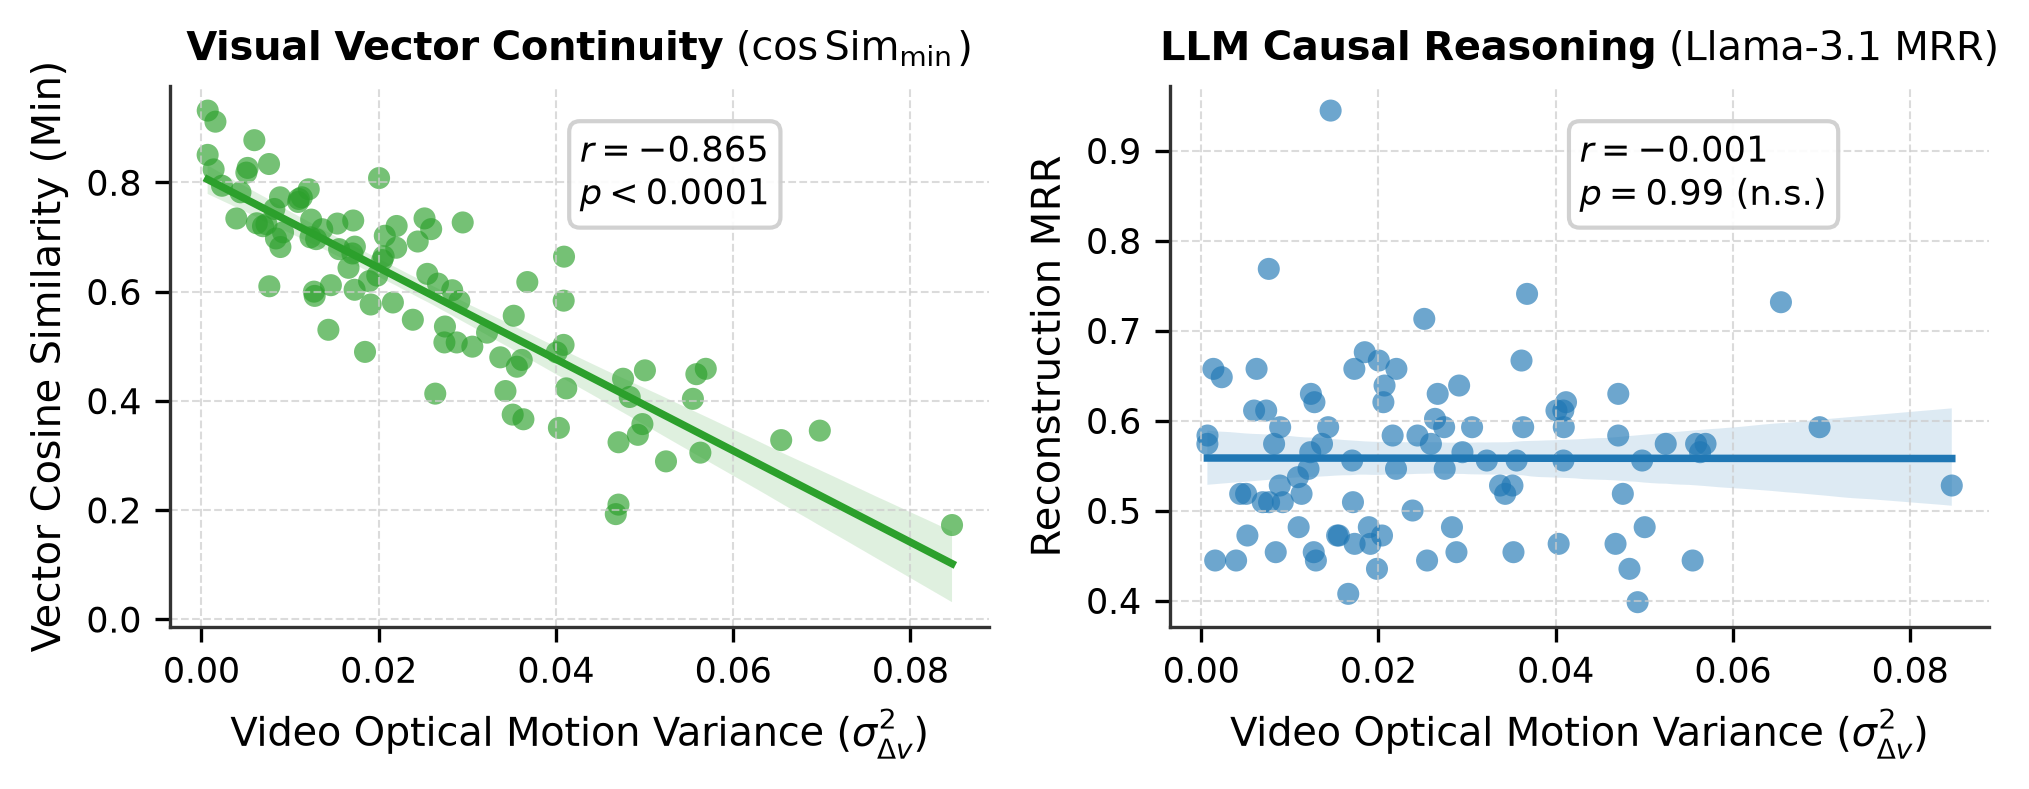
\includegraphics[width=0.98\textwidth]{figures/fig2_modality_decoupling.png}
  \vspace{-2mm}
  \caption{\textbf{The Modality Decoupling Law.} (Left) Visual vector continuity degrades precipitously as optical motion variance (\(\sigma^2_{\Delta v}\)) increases (\(r = -0.865, p < 0.0001\)). (Right) LLM causal reasoning (Llama-3.1 MRR) is completely invariant to optical motion dynamics (\(r = -0.001, p = 0.99\)), establishing that language models deduce narrative progress independently of camera shake.}
  \label{fig:modality_decoupling}
  \vspace{-3mm}
\end{figure*}

\subsection{A Priori Informational Metrics}
To diagnose when and why reconstruction succeeds, we establish two modalities of a priori properties:

\noindent \textbf{A Priori Caption Surprisal (APCS):} We compute the average cross-entropy negative log-likelihood (NLL) and perplexity of the ground truth captions under a causal language model:
\begin{equation}
    \text{APCS}_{\text{NLL}} = -\frac{1}{N}\sum_{i=1}^N \log P(w_i \mid w_{<i})
\end{equation}
High APCS indicates rare vocabulary, complex phrasing, or unexpected semantic transitions.

\noindent \textbf{Visual Optical Motion Dynamics:} We quantify optical instability between consecutive video frame embeddings:
\begin{equation}
    \Delta v_t = \|v_{t} - v_{t-1}\|_2, \quad \sigma^2_{\Delta v} = \text{Var}(\{\Delta v_t\}_{t=2}^T)
\end{equation}
where \(\sigma^2_{\Delta v}\) captures visual motion variance, abrupt cuts, and high-frequency camera transitions.

\subsection{Post-Reconstruction Evaluation}
For each missing segment \(t \in M\), we evaluate candidate retrieval over the universe of video segments \(\mathcal{U}\). The model ranks candidates by cosine similarity:
\begin{equation}
    \text{Sim}(e_1, e_2) = \frac{e_1 \cdot e_2}{\|e_1\| \|e_2\|}
\end{equation}
We report \textbf{Mean Reciprocal Rank (MRR)} (\(\frac{1}{|\mathcal{U}|} \sum \frac{1}{\text{Rank}}\)), \textbf{Recall@1}, and both \textbf{Mean} and \textbf{Minimum Cosine Similarity} (\(\cos\text{Sim}_{\min} = \min_{t \in M} \text{Sim}(\hat{e}_t, e_t^*)\)).

%-------------------------------------------------------------------------
\section{Experiments and Results}
\label{sec:experiments}

\subsection{Benchmark Dataset}
We evaluate on 100 wild videos sampled from the WildQA corpus~\cite{castro-etal-2022-in-the-wild}, spanning six diverse categories: \textit{Farming}, \textit{Survival}, \textit{Military}, \textit{Action/Vehicle}, \textit{Nature/Documentary}, and \textit{Scenery}. Each video contains dense 3-second interval annotations. We evaluate across a continuous masking width of \(W=3\) (a 9-second narrative omission), with evaluation instances placed across Opening (\(i=0\)), Middle, and Ending segments, yielding 300 reconstruction episodes.

\begin{table}[t]
\centering
\footnotesize
\setlength{\tabcolsep}{1.8pt}
\caption{\textbf{Statistical Correlation Matrix} between a priori properties and post-reconstruction metrics across 95 fully cross-evaluated videos. Pearson \(r\) and Spearman \(\rho\) (*: \(p < 0.05\), **: \(p < 0.01\), ***: \(p < 0.001\), ns: not significant).}
\label{tab:correlations}
\begin{tabular}{llcccc}
\toprule
\textbf{Prior Metric} & \textbf{Post Metric} & \textbf{Pearson \(r\)} & \textbf{Sig.} & \textbf{Spearman \(\rho\)} & \textbf{Sig.} \\
\midrule
APCS NLL & Phi-3 MRR & \textbf{-0.6408} & *** & -0.3405 & *** \\
APCS NLL & Llama-3.1 MRR & \textbf{+0.0276} & ns & +0.0365 & ns \\
APCS NLL & Llama vs. Phi \(\Delta\) & \textbf{+0.2022} & * & +0.1446 & ns \\
APCS NLL & Visual MRR & -0.1417 & ns & -0.2261 & * \\
\midrule
Motion Avg & Visual \(\cos\text{Sim}_{\text{mean}}\) & \textbf{-0.8613} & *** & -0.8617 & *** \\
Motion Avg & Visual \(\cos\text{Sim}_{\min}\) & \textbf{-0.8264} & *** & -0.8293 & *** \\
Motion Avg & Llama-3.1 MRR & -0.0808 & ns & -0.0813 & ns \\
\midrule
Motion Var \(\sigma^2_{\Delta v}\) & Visual \(\cos\text{Sim}_{\min}\) & \textbf{-0.8648} & *** & -0.8622 & *** \\
Motion Var \(\sigma^2_{\Delta v}\) & Llama \(\cos\text{Sim}_{\min}\) & \textbf{-0.3106} & ** & -0.3087 & ** \\
Motion Var \(\sigma^2_{\Delta v}\) & Llama-3.1 MRR & \textbf{-0.0013} & ns & +0.0304 & ns \\
Motion Var \(\sigma^2_{\Delta v}\) & Phi-3 MRR & +0.0290 & ns & -0.0748 & ns \\
\bottomrule
\end{tabular}
\vspace{-2mm}
\end{table}

\subsection{Finding 1: Scale-Induced Surprisal Immunity}
As presented in \Cref{fig:surprisal_immunity} and \Cref{tab:correlations}, prior caption surprisal (APCS NLL) exhibits a massive negative correlation with Phi-3-mini performance (\(r = -0.6408, p < 0.0001\), power \(= 100\%\)). Compact models lean heavily on high-probability stereotypical phrases; when real-world events diverge from standard templates, their generative capability collapses.
In sharp contrast, Llama-3.1-8B shows no significant correlation with APCS NLL (\(r = +0.0276, p = 0.7908\)). Comparing these two dependent correlations via Williams' test reveals that Llama's robustness shift relative to Phi-3 is statistically decisive (\(t = -5.51, p = 3.2 \times 10^{-7}\)). Consequently, Llama's margin of victory over Phi-3 increases significantly as caption surprisal rises (\(r = +0.2022, p = 0.0495\)).

\begin{figure}[t]
  \centering
  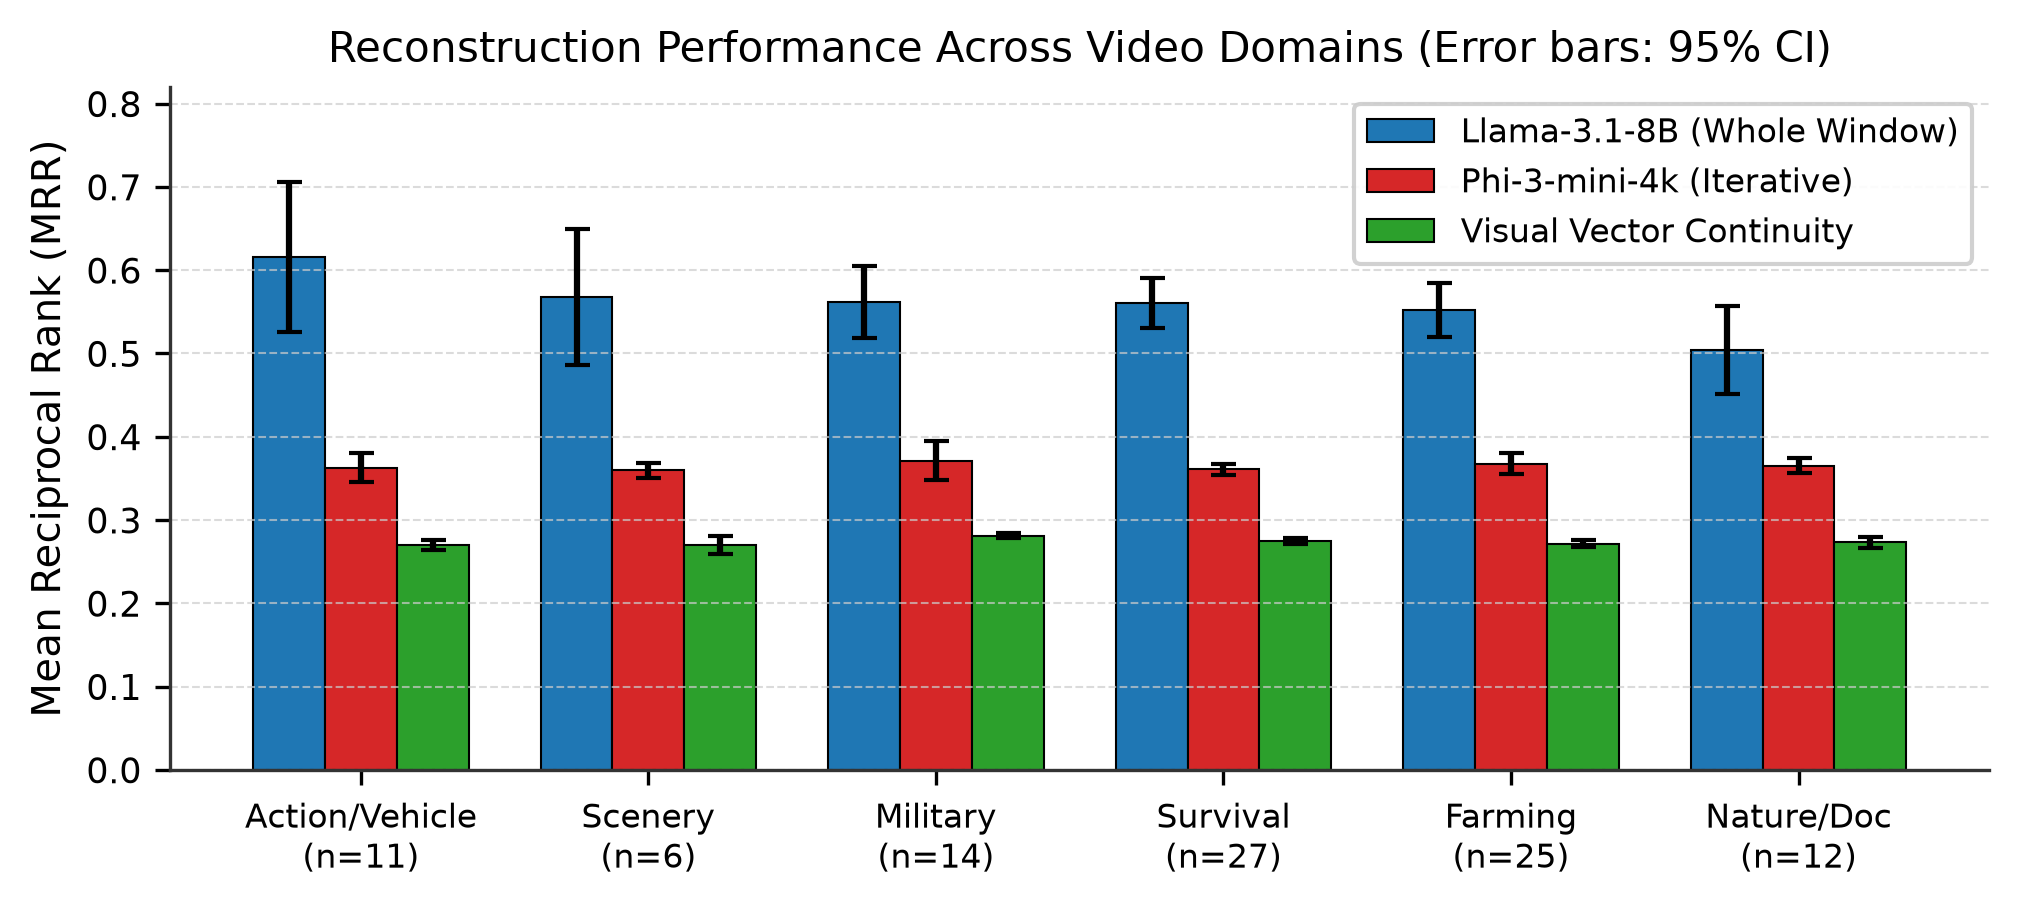
\includegraphics[width=0.98\columnwidth]{figures/fig3_category_performance.png}
  \vspace{-2mm}
  \caption{\textbf{Reconstruction Across Domains.} Error bars denote two-tailed 95\% Student's \(t\) confidence intervals. While between-category differences for Llama-3.1 are not statistically significant (\(p = 0.096\)), its paired advantage over Visual Continuity and Phi-3 is consistent across all domains (\(p < 0.0001\)).}
  \label{fig:category_performance}
  \vspace{-3mm}
\end{figure}

\subsection{Finding 2: The Modality Decoupling Law}
\Cref{fig:modality_decoupling} empirically validates the Modality Decoupling Law. For non-parametric visual interpolation, motion variance acts as an immediate failure mode: visual cosine similarity degrades dramatically with motion variance (\(r = -0.8648, p < 0.0001\), power \(= 100\%\)). When a scene undergoes rapid panning, cutting, or erratic subject displacement, visual interpolation fails because the optical manifold breaks temporal smoothness.

Language reasoning, however, is decoupled from visual motion: the correlation between optical motion variance and Llama-3.1 MRR is virtually zero (\(r = -0.0013, p = 0.9899\)). A textual description (e.g., \textit{``The combine harvester turns 90 degrees at the edge of the crop row''}) remains fully deducible regardless of whether the physical recording camera shook or hovered smoothly.

\begin{table}[t]
\centering
\footnotesize
\setlength{\tabcolsep}{2.5pt}
\caption{\textbf{Exploratory Domain Breakdown.} Performance across video categories (\(W=3\)). Between-category variation in Llama-3.1 MRR is not statistically significant (ANOVA \(F=1.94, p=0.096\)), but within-category paired gains over Visual Continuity are massive (\(p < 0.0001\)).}
\label{tab:categories}
\begin{tabular}{lcccccc}
\toprule
\textbf{Domain} & \textbf{N} & \textbf{APCS} & \textbf{Motion} & \textbf{Phi-3} & \textbf{Visual} & \textbf{Llama-3.1} \\
\midrule
Action/Vehicle & 11 & 1.168 & 0.146 & 0.363 & 0.270 & \textbf{0.615} \\
Scenery & 6 & 1.190 & 0.085 & 0.360 & 0.270 & \textbf{0.568} \\
Military & 14 & 1.112 & 0.194 & 0.371 & 0.281 & \textbf{0.562} \\
Survival & 27 & 1.073 & 0.150 & 0.361 & 0.275 & \textbf{0.560} \\
Farming & 25 & 1.024 & 0.196 & 0.368 & 0.272 & \textbf{0.552} \\
Nature/Doc & 12 & 1.223 & 0.190 & 0.365 & 0.273 & \textbf{0.505} \\
\midrule
\textbf{Overall Mean} & \textbf{95} & \textbf{1.103} & \textbf{0.165} & \textbf{0.365} & \textbf{0.274} & \textbf{0.558} \\
\bottomrule
\end{tabular}
\vspace{-3mm}
\end{table}

\subsection{Finding 3: Bottleneck Metric and Positional Teleology}
\noindent \textbf{Sensitivity of \(\cos\text{Sim}_{\min}\):} As shown in \Cref{tab:correlations}, minimum cosine similarity exhibits stronger sensitivity to motion shocks (\(r = -0.3106, p = 0.0022\)) than mean similarity (\(r = -0.2568, p = 0.0120\)). Mean similarity masks severe localized ruptures in multi-second gaps, whereas \(\cos\text{Sim}_{\min}\) accurately flags the single weakest link.

\begin{figure}[t]
  \centering
  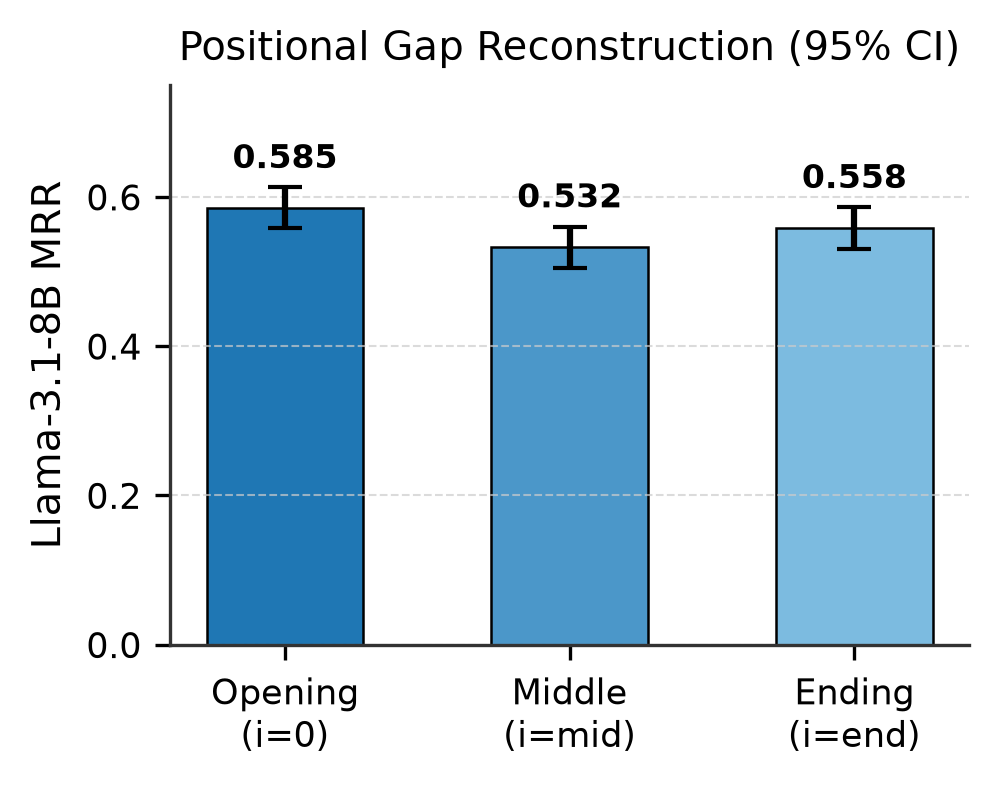
\includegraphics[width=0.60\columnwidth]{figures/fig4_positional_mrr.png}
  \vspace{-2.5mm}
  \caption{\textbf{Positional Reconstruction MRR (95\% CI).} Opening sequences (\(i=0\)) outperform middle segments (\(p = 0.0058\)), reflecting backward causal constraints in edited video.}
  \label{fig:positional_mrr}
  \vspace{-2.5mm}
\end{figure}

\noindent \textbf{Positional Teleology:} Reconstructing opening sequences (\(i=0\)) achieves significantly higher retrieval MRR (\(0.585 \pm 0.028\)) than middle segments (\(0.532 \pm 0.028\), paired \(t = 2.82, p = 0.0058\)), while the difference between opening and ending segments (\(0.558 \pm 0.028\)) is not statistically significant (\(p = 0.177\)) (\Cref{fig:positional_mrr}). In natural video editing, downstream narrative resolution is strongly determined by initial conditions; working backward from the established premise provides tighter causal constraints than forward open-ended branching.

%-------------------------------------------------------------------------
\section{Discussion and Implications}
\label{sec:discussion}

\noindent \textbf{Dynamic Multimodal Token Compression:}
Our results offer a concrete architectural design guideline for Video-LLMs: rather than allocating uniform frame tokens across time, architectures should compute local motion variance \(\sigma^2_{\Delta v}\) and caption predictability. In quiescent, low-variance intervals, visual embeddings can be compressed via simple temporal interpolation. Conversely, when visual surprisal spikes or frames are intentionally dropped for efficiency, the system should rely on symbolic language reasoning.

\noindent \textbf{The Event Horizon:}
While an 8B model successfully bridges 9-second gaps (\(W=3\)) with 0.558 MRR, future work must establish the critical gap threshold—the ``Event Horizon'' (\(W \ge 6\))—where narrative divergence turns chaotic and parametric world models can no longer constrain physical reality.

%-------------------------------------------------------------------------
\section{Conclusion}
\label{sec:conclusion}
Through dense caption reconstruction, we demonstrated that language models operate as robust causal engines capable of bridging temporal omissions in video. We established that parametric scale (\(\ge 8\text{B}\)) eliminates vulnerability to language surprisal, and proved that symbolic reasoning is mathematically decoupled from optical motion disturbance. These principles pave the way toward selective, semantically guided video processing architectures.

{\footnotesize
\setlength{\bibsep}{0pt plus 0.3pt}
\bibliographystyle{ieeenat_fullname}
\bibliography{main}
}

\end{document}
